% \documentclass[a4paper,12pt,titlepage]{article}
\documentclass[runningheads]{llncs}
\setlength{\parskip}{1em}


%Bibliography
\usepackage[natbib=true, citestyle=apa, bibstyle=apa]{biblatex}
\bibliography{ToBITEnglishCorrectionSoftware.bib}

\usepackage{csquotes}
\usepackage{enumitem}
\usepackage{todonotes}
\usepackage{xspace}
\usepackage{dirtytalk}
%Manage graphics%
\usepackage{graphicx}

\usepackage{float}

\let\OldTextregistered\textregistered
\renewcommand{\textregistered}{\OldTextregistered\xspace}%
%\usepackage[utf8]{inputenc}
%\usepackage[english]{babel}
%\usepackage{blindtext}
%\usepackage{microtype}
%\usepackage{graphicx}
%\usepackage{wrapfig}
%\usepackage{fancyhdr}
%\usepackage{amsmath}
%\usepackage{index}
%\usepackage[onehalfspacing]{setspace}
%\usepackage{nomencl}
%\makenomenclature
%\renewcommand{\nomname}{List of Abbreviations}

%opening

%\makeindex

\begin{document}

%\title{\Large{\textbf{English Correction Software}} }
\title{English Correction Software}
\subtitle{ToBIT Paper}

\author{Tobias Koller}

\institute{University of Applied Science Northwestern Switzerland (FHNW), \\ 4000 Basel, Switzerland}


\maketitle              % typeset the header of the contribution


\begin{abstract}
This paper forms ....

\keywords{Grammarly\textregistered \and Natural Language Processing \and Language Correction Software}
\end{abstract}


%\let\cleardoublepage\clearpage
%\pagenumbering{roman}

\section{Introduction}
Numerous software solutions on the market promise to help in particular non-native English speakers with grammatical error detection and improving the style and structure of their writing. In the course of the module ``Innovative Topics in Business Information Technology'' (ToBIT), I am going to evaluate different products regarding their functions, ease of use and effectiveness in supporting the writing process. The main goal is to use literature review to discover how effective the correction software is under real conditions.

One widely known and used writing tool for grammar checking, spell checking, and plagiarism is Grammarly\textregistered®. Since it is one of the leading products in this field and there are innumerable research papers to support, I focus on this particular tool.

After the evaluation of the tools, I will also describe different natural language processing (NLP) techniques that are being applied. In the final part of the document, the findings will be discussed to show clearly the current state of the art in this field. A recommendation to the University of Applied Sciences and Arts Northwestern Switzerland (FHNW) will be given on what products to consider or how to develop a new product internally.

\pagenumbering{arabic}

\section{Existing solutions}
\subsection{Grammarly\textregistered}
Grammarly\textregistered, a company with its eponymous popular language correction software, aims to \textquote[{\cite{noauthor_write_nodate}}]{help people improve their communication}. Max Lytvyn, Alex Shevchenko, and Dmytro Lider founded the company 2009 with a strong focus on supporting the student's writing process. In the meantime, they broadened their scope to businesses as well as private customers. Grammarly\textregistered @edu and Grammarly\textregistered business both meet the need of each of these customer segments. Their correction service is based on analysing the written content in real-time while showing suggestions in the form of correction cards that can be accepted or rejected. To promote the writer's learning progress, further grammatical information regarding the specific issue can be retrieved from the card which can help to decide on whether to accept the changes or not. \citep{noauthor_write_nodate}

Being a successful grammar checker requires to be available where people create texts. These places are as diverse and multi-faceted as the client groups. While academic and business end-users might use predominantly classical text processing software, most pirvate users need the grammar support in their browser (web forums, social media) and increasingly on their mobile devices (chats, e-mails). Grammarly\textregistered responds to this with various products. Browser plugins for all major browsers (Chrome, Safari, Firefox, Edge) provide accompanying grammar service during your browsing experience. Input text fields are automatically detected and errors are highlighted with the option to see the correction card. Users of Windows and Mac can download a Grammarly\textregistered text editor, but similar functionality can also be used in their web application on app.grammarly.com. To also serve customers who write on mobile devices, the Grammarly\textregistered team developed a keyboard for Android and iOS. For both Microsoft Word and Outlook, Grammarly\textregistered provides a special plugin that integrates directly and seamlessly with the writing process.

Writers can expect three different types of support from the software. According to their webpage \parencite{noauthor_write_nodate} support ranges from grammar checking, tone detector and for paying users even a plagiarism checker. They claim that their grammar checker does not only find misspelt words but also recognises comma and other punctuation errors. Furthermore, their premium service includes more advanced suggestions to enhance the writing style. Assistance in appropriate language style is given by defining so-called goals on which the algorithm bases its recommendations on. Parameters that can be predefined include target audience, formality, domain and tone of writing.   

Use of the base functionality is free but requires registration. This may lower the entry threshold since all that is required is an e-mail address and a computer or smartphone with an internet connection. However, a premium service is offered against payment. Grammarly\textregistered's website \citep{noauthor_write_nodate} shows the deviation from the premium plans to the free version. The plans ``Premium'' and ``Business'' both comprise the same advanced features including grammar correction in the following categories.
\begin{itemize}
 \item Fluency
 \item Readability
 \item Engagement
 \begin{itemize}
  \item Compelling vocabulary
  \item Lively sentence variety
 \end{itemize}
 \item Delivery
 \begin{itemize}
  \item Confident language
  \item Politeness
  \item Formality level
  \item Inclusive language
 \end{itemize}
 \item Plagiarism detection
\end{itemize}
``Business'' plan only differs in the account management tools that are available to the organisation's administrator as well as business-oriented billing. The available software and plugins (browser, MS Word, MS Office, mobile keyboard) are equally available in the paid and free subscription model. Since Grammarly\textregistered has its focus on supporting students, they target educational institutions with their programme ``grammerly@edu''. The grammar checking functionalities seem to be the same as in the ``Premium'' and ``Business'' plans but they offer specialised licenses and 24/7 support. Different versions of the same tool make the evaluation of the tool in the following chapter more difficult since some of the research found is based on the limited functionalities. Furthermore, the software developed greatly in the past years as can bee seen on print screens from \textcite{dembsey_closing_2017}. This needs to be taken into account when judging the results from this analysis.


\subsection{Criterion\textregistered}
The online writing evaluation service named Criterion\textregistered is specially tailored to be used in schools and universities and focuses on the tasks of automated essay scoring and improving student's writing skill by use of automated feedback but also facilitating the revisioning process online. The software is developed by Educational Testing Service (ETS) \citep{noauthor_ets_nodate}.

This focus on institutions can be recogniced when visiting their webpage \citep{noauthor_ets_nodate}. In order to get hands on the tool you need to login through your organisation. Private users are excluded from the potential customers. 

According to \textcite{lim_review_2012} using Criterion\textregistered usually starts with the teacher setting-up an assignment for his class. He as ample parameters to tailor the assignment to his needs, like a category (level of writing), different topic modes and an essay topic. Criterion\textregistered comes with a library of predefined essay topics for which there is a cataloque of past scripts written by former students and scored by human raters. This collection is later used to evaluate the student's work by comparing them to the already scored scripts. The teacher can run the assignment as a test and impose a time limit or decide to give unlimited time (for learning and practice). Furthermore, the teacher can set the number of possible re-submissions, the categories that should be displayed to the student and the deadline for submission. While the assignment is ongoing the teacher has its own dashboard to supervise the progress of the class or each individual student. Additionally to the feedback provided by Criterion\textregistered the teacher can add personal feedback manually. Teachers and students can discuss directly via the Criterion\textregistered web platform which allows them to directly comment on certain passages of the text. After the submission by a student, he is presented with an overall score and an overview of the errors detected including a detailled description of those.

\subsubsection{E-rater}
The evaluation engine behind Criterion\textregistered is named e-rater\textregistered. As detailled by \textcite{lim_review_2012} e-rater\textregistered bases its scoring on a statistical approach by analysing previously graded essays. An overall of 11 features are being detected and compared to the evaluated dataset. By use of linear regression the score is then predicted. It is important to notice that e-rater\textregistered is trying to mimic human scorer and can therefore, by definition, never overtake the scoring quality of human beings. 


\section{Evaluation}

\subsection{Grammarly\textregistered}
Grammarly\textregistered's web presence \citep{noauthor_write_nodate} makes strong claims about the effectiveness and usefulness of the system. Over the past years, several researchers attempted to measure the impact of using Grammarly\textregistered on student's written performance and determine the overall quality of the feedback produced \citep{dembsey_closing_2017,nova_utilizing_2018,ventayen_graduate_2018}. Others \citep{cavaleri_you_2016} aimed to determine the perceived ease of use and perceived usefulness in order to answer the question whether the technology will be accepted or not. The methods used include comparing Grammarly\textregistered's machine-generated feedback to the feedback provided by online writing consultants \citep{dembsey_closing_2017}, comparing students' performance in language tests before and after being exposed to the software \citep{qassemzadeh_impact_2016} and different kinds of surveys and questionnaires \citep{nova_utilizing_2018, cavaleri_you_2016, ventayen_graduate_2018}.

\subsubsection{Quality of feedback}
Feedback provided by a grammar correction software should be understandable by the end-user to promote learning. Simply accepting suggestions of the software blindly does not support avoiding the mistake in the future. Additionally, the correction algorithms are not flawless and their proposed changes should always be questioned. This is only possible if the writers understands the issue that was found in their writing \citep{dembsey_closing_2017}.

A clear understanding of the problem described and the terminology used in the feedback is required for a student to derive learning gains. In the field of linguistics specialised terminology is being used to describe sentence structures. Especially for students of English as a foreign language (EFL), those terms might be ambiguous and need further explanation. \textcite{dembsey_closing_2017} found that Grammarly\textregistered used 52 different terms from the linguistic vocabulary in the correction of three essays while on the other hand, 10 online writing consultants used only 32 terms (all consultants combined), or 10 terms on average, for the same documents. Furthermore, the consultants used much more accessible language in their comments and even attempted to use the student's own language to give more comprehensible feedback. Giving feedback in an appropriate format for the receiver can be achieved by humans better than by algorithms. In general advanced terminology is not supportive for the learning process of the student. Simple language should be used whenever possible \citep{dembsey_closing_2017}.

In the best case, the grammar correction software's feedback encourages the user to scrutinise the passage containing an issue and give some valuable recommendations to improve it. However, if the issues are not correctly detected, the feedback can mislead and confuse the writer. In an interview conducted with Indonesian EFL postgraduate students \citep{nova_utilizing_2018}, multiple participants reported that Grammarly\textregistered changed the sentence's intentional meaning, thus leading to their confusion. As long as students are aware of the software's mistake, they can simply ignore it and proceed. More harmful are those incidents when the student is at a beginner's level in English. Students lacking language experience are more tempted to accept proposed corrections without spotting the erroneous suggestions. As \textcite{vojak_new_2011} point out such a situation of uncertainty is counterproductive to the author's development of confidence in his writing. The notion of something being wrong disencourages creative writing and instead motivates to comply with standard language patterns und generic phrases. Instead of promoting better writing style, they \textquote[{\cite{vojak_new_2011}}]{fear that the persistent underlying urge towards conformity may stifle individual creativity}. 

Grammar correction on a sentence level follows rather clear rules whereas connections within a paragraph or even the logical structure of the whole document are much more sophisticated tasks. Unsurprisingly automated correction software like Grammarly\textregistered has its difficulties. Students experienced the lack of context-aware checking such as examining the text for coherency and cohesiveness. Those who needed the software only to check the grammar did not find this an issue \citep{nova_utilizing_2018}. The same results were found by \textcite{dembsey_closing_2017} who observes that Grammarly\textregistered treats each word and sentence individually and does not make any connections between them, therefore drastically reducing the learning opportunity compared to expert feedback.


\subsubsection{Amount of errors found}
The quantitative figure of detected errors is not sufficient to demonstrate the superiority of a correction algorithm. As a result of the comparison between Grammarly\textregistered's and writing consultant's analysis of three student essays, \textcite{dembsey_closing_2017} observed a total of 118 issues whereas the cumulative average of the 10 consultants only identified 51. Repetition of the same issues was the main driver for such a high number of detected issues. A human proofreader could encourage the student to look for additional instances of the same mistake by themselves, leaving more room in the coaching session to address different issues. To get a better view of the issues discovered, all issues were categorised which led to a total of 16 categories to which every issue could be assigned. In all the essays combined Grammarly\textregistered's correction cards could be assigned to only six types of issues. This again shows the rather narrow range of recommendations. Cumulated all 10 consultants addressed 15 issue categories and even on average they addressed more (8) diverse topics than Grammarly\textregistered.

Despite having found more issues than a human proofreader, Grammarly\textregistered's issue detection was highly repetitive and only addressed a narrow range of issues. The consultants used less comments but gave a more in-depth explanation and could even connect sentence-level issues to general (thesis) level issues. Furthermore, a high number of issues is often not beneficial for the learning rate of students, as they might become intimidated and demotivated. 
\citep{dembsey_closing_2017}


\subsubsection{Accuracy}
A more crucial measure of value provided by the feedback than the number of issues detected is the accuracy of the results. False positives are reported issues that are no problems at all. \textcite{dembsey_closing_2017} also considered incorrect use of term or incorrect explanation as an inaccuracy. 41\% of Grammarly\textregistered's correction cards were inaccurate, either representing false positives or using wrong terms for the specific issue. At the same time, consultants only had an average inaccuracy of 10\% which originated mostly from using wrong terms.
\citep{dembsey_closing_2017}

The decision whether an issue should be raised or not is also dependent on the type of writing. This puts an automated correction software in a disadvantageous position, since detecting type of writing as well as target audience is generally difficult. \textcite{cavaleri_you_2016} tested Grammarly\textregistered's premium version and could indicate the type of writing. For ``essay'', ``dissertation'', ``presentation'', ``blog'', ``business document'' or ``creative writing'' different rules of raising issues would be applied. This improved the accuracy of the feedback profoundly.

At the moment of writing, Grammarly\textregistered also allows setting some meta information to the document allowing for increased accuracy. Audience (general, knowledgeable, expert), formality (informal, neutral, formal), tone (neutral, confident, joyful, optimistic, friendly, urgent, analytical, respectful) and intent (inform, describe, convince, tell a story) are available in the free version. The latter two are marked as experimental. Only the domain (academic, business, general, technical, causal, creative) is available in the premium version. The fact that they decribe these features as experimental, shows that Grammarly\textregistered has already detected the necessity to increase accuracy employing better discourse analysis.

\subsubsection{Perceived Ease of use}
For a correction software to be used as part of the student's writing process, it must be simple and intuitive. These are non-functional requirements and therefore more difficult to measure. The literature found focuses on the perceived ease of use reported by students using the tool.

In the Pangasinan State University, \textcite{ventayen_graduate_2018} conducted a usability study employing a SUS (System Usability Scale) and detected an average usability score of 86.04\%. Students found it very easy to use the system and even thought that most people would learn to interact with the system very quickly. In a survey \citep{cavaleri_you_2016} conducted in an Australian college, 94.4\% of the students rated the ease of use of Grammarly\textregistered with 4 or 5 with 5 being 'extremely easy'. Only one out of 18 students reported having technical issues using the system. Negative statements about the ease of use were made about the automatic detection of Australian or American grammar and spelling. The tool did not allow the manual selection of language and the detection did not always work. Furthermore, some students found it difficult to navigate the page.

Easiness of access to the tool was also be considered. This includes especially the barriers that need to be overcome before the actual usage of the system can take place such as registration, download and installation. The only requirement to start using Grammarly\textregistered is the registration with an e-mail address and password. Technically the installation of any software is not required since the system can be used immediately through the browser which gives access to the grammarly application \citep{noauthor_write_nodate}. The features are better integrated into the writing process when the provided plugins are used. The interviewed students in \citeauthor{nova_utilizing_2018}'s study found no barriers in the download and setup process.

\subsubsection{Perceived Usefulness} 
According to the Technology Acceptance Model (TAM), besides ease of use, perceived usefulness is a key factor that influences people's intention to use computer systems \citep{davis_user_1989}. In the survey conducted by \citeauthor{cavaleri_you_2016} \textquote[{\cite{cavaleri_you_2016}}]{most students reported that they found the suggestions helpful for improving the particular paper they had submitted to Grammarly\textregistered and half felt it helped them achieve a better mark}. Effects were not only short term, students felt the card's feedback helped them in understanding issues better and in improving their writing skills also long-term. Therefore, usefulness is not limited to the current piece of writing but rather applies to the whole learning experience of each user and supports self-directed learning. Besides the direct improvements on the correctness of the grammar, 77.8\% of respondents felt an increase in their confidence level after using Grammarly\textregistered. 

These results corroborate the conclusions of students interviewd by \textcite{nova_utilizing_2018}. They mention the positive impact of feedback cards on their self-revision. Increased reflection on the detected issues helped them to improve the quality and avoid the repetition of errors. Especially the indication of example sentences helped them to understand the issues better and apply a correction.

However, some students also identified disadvantages that reduced the overall usefulness of Grammarly\textregistered. Both \textcite{ventayen_graduate_2018} and  \textcite{nova_utilizing_2018} claimed that some parts of the document should be excluded from grammar checking such as the bibliography that follows certain standards. Checking on a reference list does not yield any benefit and only distracts \citep{ventayen_graduate_2018, nova_utilizing_2018}. Another limitation found by \textcite{cavaleri_you_2016} was the complex language used in some of the recommendations. Deciding on whether to accept the change or not required some deeper understanding of the problem at hand. When students were not able to understand the issue and the underlying grammar rule, they were not able to make those decisions. Therefore, advanced English writers could benefit more than others. The complex language used in the feedback cards can be seen as a barrier for beginner-level students. 

\subsection{Criterion\textregistered}
As the underlying engine of Criterion\textregistered uses human evaluated texts as a basis, the evaluation of its fit should be determined by the degree it resembles human raters. \textcite{weigle_validation_2010} validated that the scoring of a human evaluator and e-rater\textregistered do correlate. \citeauthor{lim_review_2012} state \textquote[{\cite{lim_review_2012}}]{that the correlations between e-rater and human ratings were indistinguishable from those between two humans’ ratings, suggesting that the two different rating procedures are measuring writing equally well. } However \textcite{lim_review_2012} also detect the limitations of the tool. The statistical method chosen puts a high focus on the quality and the linguistical accuracy but fails to value the strong argumentation and coherence. 

\subsection{AWE application in classrooms}
\subsubsection{Automatic Writing Evaluation}
Automatic Writing Evaluation (AWE) programmes are specially designed for the application in the classrooms where students write reports and essays. They use  \textquote[{\cite{grimes_utility_2010}}]{artificial intelligence (AI) to score stu-
dent essays and support revision}.
The features of such an AWE are usually tailored to the use case of a class, providing the student with the option of submitting the paper for grading. Before final submission, the student usually has the opportunity to go through several revisions and receive automated feedback by the AWE. Eventually, the grading can also be done by the AWE or support the lecturer in this task. Such a system can accomplish more revisions of a student's document than a human can do because of capacity restrictions \citep{warschauer_automated_2006}. \textcite{grimes_utility_2010} state the limited capacity of teachers in English language arts is the main bottleneck on the feedback they can provide to their students and consequently their development of writing skills. AWE is often seen as the silver bullet that solves all these problems. Removing this bottleneck would allow for more revisions, more writing practice and as a result more motivation by students to write and revise.        

How is this technology being applied in these days classrooms and how effective is it supporting the learning goals? In a multi-year study, \textcite{grimes_utility_2010} observed the attitude of students and teachers towards this new technology. 

\subsubsection{Teacher's attitude towards AWE}
Incorporating an AWE system comes with a change in the structure of writing classes and the role of the teacher. When working with AWE the teacher became more of a supervisor who was present to help the students with the usage of the system or to answer questions. Their role shifted from judge to a supportive coach with whom the students wanted to collaborate. This was only possible since the judgement of the writing was offloaded to a machine which distanced the teacher from his role as a rater and the students sought advice for improvement from a third party \citep{grimes_utility_2010}. This made the management of a class much easier. Students tended to be more autonomous and self-motivated when working with AWE and their reluctance to write decreased significantly. Teachers saved a lot of time they would otherwise have spent on low-level issues. This allowed the teacher to put their focus on high-level concerns like the style and overall structure since low-level grammatical errors were taken care of by the system.

The participating schools in the study by \textcite{grimes_utility_2010} were using the AWE named ``My Access'' (MA) which offers an automatic scoring feature. The score will be visible by both the teacher and the student and students can do further revisions by working on the feedback given by MA. The final grade was still determined by the teacher but influenced by the score given by MA. Teachers indicated that the grade given was influenced by MA by an average of 18\%. This number is relatively low since most teachers did not put much confidence in the accuracy and fairness of the automated scoring. On average they treated the fairness of the system slightly lower than neutral. Knowing the limitations of the automated scoring it is not surprising that teachers still read the students work very thoroughly. 41\% reads them even as thoroughly as when they would not use MA. 

Teachers observed different reactions to the automated scoring feature \citep{grimes_utility_2010}. While some students were increasingly motivated to write a high-quality text for the immediate reward others were highly distracted by the score and could no longer focus on their task. Some teachers even disabled the automated scoring and only showed it to their students after submission. Some of the high-performing students that reached a very high score on their first submission were no longer motivated to complete revisioning whereas if they would not have known they could have still found parts to improve. Another development observed was students that tried to learn how the scoring algorithm works and then submit text that would simply lead to a higher score but does not make sense in the context of the paper. From those reports, it can be concluded that teachers are advised to tightly observe the usage of the AWE by their students. Only if they support their students and prevent misuse the automated scoring can provide real value by allowing the writers to assess and motivate themselves.

\subsubsection{Student's attitude towards AWE}
Increased motivation towards writing and revising was found by \textcite{grimes_utility_2010}. Reasons identified were the immediate feedback by the AWE instead of week-long waiting time for a human feedback. For them, the automatic score seemed to have the characteristics of gamification. As a result they tried to outperform each other which increased motivation even further. They were also able to use the time after the first submission for further improvements since the feedback is available immediately.

Students also did not rate the fairness of the automatic grades as critical as the teachers. They rated the fairness with 3.4 (on a 5-point scale) whereas the teacher's rating was only 2.8.

Regarding the amount of revisions done by students, the first year did not show any increase and only 12\% of essays had more than one revision \citep{grimes_utility_2010}. In the following year, this changed to 53\%. On the one hand, it can be reasoned that teachers allocated more time for the revision process but also the students who learned how to properly use the system and make the best use of its features. Students who revise their writings first focus on low-level issues like spelling and punctuation before moving to feedback about organisation and development. This seems to be a natural behaviour to focus on the low-hanging fruits that can be fixed with lower efforts. Improving on the structure takes much more time and often requires reading large parts again to come up with a strategy to re-arrange it.

\subsubsection{AWE usage} After looking at both the teacher's and the student's side it can be concluded that AWE usage can remarkably improve the learning process. More time is available to focus on higher-level concerns like organisation and development since issues in spelling, punctuation, grammar and word choice were taken care of by the software. Overall student motivation significantly increased. According to \textcite{grimes_utility_2010} this need to be taken with care. The higher motivation observed was mainly based on the goal to reach a high score, not mainly to write better texts and learn from it. This shift from internal to external motivators is not beneficial to the students. Furthermore, students must be closely observed when using AWE and teachers need to take appropriate actions when they see problems. Not all students interact equally with this new support. Some might be distracted by the scoring while others lose motivation after receiving a good initial score. \citeauthor{grimes_utility_2010} concludes that there is a need for \textquote[{\cite{grimes_utility_2010}}]{sensible teachers who integrate AWE into a broader writing program emphasizing authentic communication, and who can help students recognize and compensate for the limitations of software that appears more intelligent at first than on deeper inspection.}.

\vspace*{6mm}\hspace*{6mm} \textit{AWE effectiveness studied with control group in \cite{wang_exploring_2013}}  \par


\section{Techniques of natural language processing}
briefly explain difference between Grammatical error detection (GED) and grammatical error correction (GEC) by \cite{bell_context_2019}.

\subsection{Part of speech tagging}
Different techniques used for GED and GEC make use of part-of-speech (POS) tagging. During this process every word of a sentence is assigned a tag of its grammatical category \citep{noauthor_pos_2018}. The different tags used are defined in the tagset. They can vary by the degree of detail. Basic tags only distinguish between noun, verb, adjective, etc. while others distinguish male/female, plural/singular, tense and person. This tagging alone does not yet give any insight into the correctness of a sentence, it simply gives insight about the structure of a sentence and the role of the words in it. This then allows automated text processing software to do further analysis.

\subsection{Syntactic parser}   
The rules that describe the structure that a sentence has to conform with, are referred to as the syntax of a language. To detect ill-formed sentences the syntactic parsing can be applied. As a first step POS tagging needs to be applied to know about the structure of the sentence. In the next step the sentence is parsed by means of predefined constraints which resemble the rules of the specific language. According to \textcite{manchanda_various_2016} the sentence is matched with the given tree structures. If the sentence can matched with the constraints available the parsing succeeds and the sentence is syntactically correct. Failure of the parsing process simply tells that there is some syntactical error present, but does not reveal any further information.

\textbf{\textit{Example 1:}} Constraint: subject-verb agreement for number and person. Sentence: ``\underline{He} (3rd person sg.) \underline{is} tall''. Result: Constraint matches.

\textbf{\textit{Example 2:}} Constraint: subject-verb agreement for number and person. Sentence: ``\underline{He} (3rd person sg.) \underline{am} tall''. Result: Constraint does \textbf{not} match.

\subsubsection{Constraint relaxation}
In its basic form syntactic parsing only fullfills the role of grammer error detection but fails to provide insightful advice to the author. To do so, a diagnosis technique can be applied. The most widely used, constraint relaxation, is described here in more detail. In syntactic parsing the matching of partial structures is only allowed if the constraints are met \citep{vandeventer_creating_2001}. In constraint relaxation some of the constraints present are relaxed, meaning that a partial structure is allowed to match even if this constraint is violated. To give useful information to the user the relaxed constraint needs to be labelled while defining them. 

\textbf{\textit{Example:}} Constraint: subject-verb agreement for number and person. Sentence: ``\underline{He} (3rd person sg.) \underline{am} tall''. Result: Constraint matches because it is relaxed. \textbf{Label:} Verb does not correspond to the subject.

The main advantage of constraint relaxation in syntactic parsing is that it provides the full analysis of the structure and at the same time diagnoses the violations to the underlying syntacic constraints \citep{vandeventer_creating_2001}. The problem with this approach is the memory intensive computing. This is due to the fact that every correct sentence does not only match with the correct structure but also with all the relaxed versions of that structure. Additionally, the constraints of parsing are manually assembled which represents a labor intense task. 

\subsection{Statistical technique}
The statistical approach also makes use of the POS representation of a sentence. Other than the syntactical approach it does not depend on predefined rules, instead it learns from POS-annotated corpus \citep{manchanda_various_2016}. The decision whether a sentence is well-formed or not depends on the statistical measures of the frequency of those POS sequences in the corpus. It is therefore crucial that corpus of language is well chosen for the task. This means that different types of writing may need different text corpora. Different language differy widely in the sequences of POS considered as correct, which requires also seperate annotated corpora.

Great advantage in this procedure is the irrelevancy of any hand-crafted rules. A large enough POS annotated corpus is sufficient to achieve the desired results. However, the occurences considered as incorrect based on non-occurence in the corpus cannot be explained. The author is left uninformed about the reason for the detected error. This disadvantage can be mitigated by building the model not only with the POS tagged features but add a lexical feature-set \citep{gamon_using_2009}.

\subsection{Rule based technique}
The rule based technique requires the composing of a collection of error rules \citep{manchanda_various_2016}. These rules describe errors by use of POS tags that are expected to occur in the text. For every possible error an individual rule must be manually constructed. It is self-evident that this technique will never lead to a complete set of rules, since the types of erroneous senteces is innumerable. As the rules are specifically constructed for a type of error it is simple to add a detailed description with a suggestion how to fix it supplemented with the affected grammar rules.

One variation of this rule based technique does not require the definition of each individual error but allows the matching of whole error types by usage of regular expressions in n-gram templates \citep{kantrowitz_method_2003}. An n-gram is a sequence of n words in a sentence that is matched against the set of rules. The regular expressions are used so that not all the characters of a word must match the rule. This invention allows the replacement of the illegal n-gram with a legal one as the following examples illustrate:

\textbf{\textit{Example 1:}}
\newline Rule: fuly\$ $\rightarrow$ fully
\newline\textbf{illegal n-gram}: hopefu\textbf{l}ey
\newline\textbf{replacement:} hopefu\textbf{ll}y
\newline(\$ represents the end of the word)

\textbf{\textit{Example 2:}}
\newline Rule: their seem $\rightarrow$ there seem
\newline\textbf{illegal n-gram}: the\textbf{ir} seems to be...
\newline\textbf{replacement:} the\textbf{re} seems to be...

This kind of matching allows to cover numerous common errors with just one rule. The replacement of the error is then done in a context specific fashion since only errors in the specified n-gram are being replaced. This approach does not find all errors but if an issue was detected has a high certainty for a replacement and does not introduce new errors. Therefore, this technique is specially useful for automated replacements.


\section{Self experiment}
In a self-conducted experiment I want to find out first-hand how helpful the grammar correction of Grammarly\textregistered is. Grammarly\textregistered is designated for this experiment since it is easily accessible in its free version and they use advanced machine learning and deep learning techniques to improve their products \citep{noauthor_write_nodate}. The experiment should answer the following questions:

\begin{itemize}
 \item How is the user experience when revising issues with Grammarly\textregistered web?
 \item Is the feedback provided by Grammarly\textregistered understandable?
 \item Does Grammarly\textregistered help build new knowledge that later can be applied?
\end{itemize}


\subsection{Method}
In order to get a more objective result a survey paper of a fellow student is used, isntead of any product that was written by the author of this document. The paper chosen is in an early draft stage with almost no revision made. This should yield in a broad detection of different issues. The Grammarly\textregistered web based editor is used to conduct the test. The goals of the writing can be manually configured, the following settings have been made:

\begin{itemize}
 \item \textbf{Audience:} Expert
 \item \textbf{Formality:} Formal
 \item \textbf{Domain:} Normal (cannot be changed in the free version)
 \item \textbf{Tone:} Analytical
 \item \textbf{Intent:} Inform, Describe
\end{itemize}

Only a subsection (2 chapters) of a total length of 2667 words have been submitted for evaluation.

\subsection{Result}
Within less than a minute after pasting the content to the browser the calculation has already been finished. The sidebar on the right gives an overview of all the issues found. It prominently mentions that 68 alerts have been detected, but there are 90 more issues present which are only accessible in the premium version of Grammarly\textregistered. Those 68 alerts are subdivided into the two cateogries \textbf{Correctness} and \textbf{Clarity}. A progress bar also indicates the achievement of the two other cateogries \textbf{Engagement} and \textbf{Delivery}. If one wants to see how to improve and selects the category, they also mention to buy premium service first. Additionally an overall score of 48 (out of 100) is displayed.

The revision screen of Grammarly\textregistered is devided in three columns. The first column (from left to right) shows the text that is being edited at the moment. Issues are highlighted by underlining the sections in a specific color. Each of the before mentioned issue categories is assigned to one color. The second column shows a feedback card for each issue. They appear on the same height as the is located in the first column. While scrolling through the page they are synchronised. The last column  is the sidebar that was already described before. 

\begin{figure}[H]
  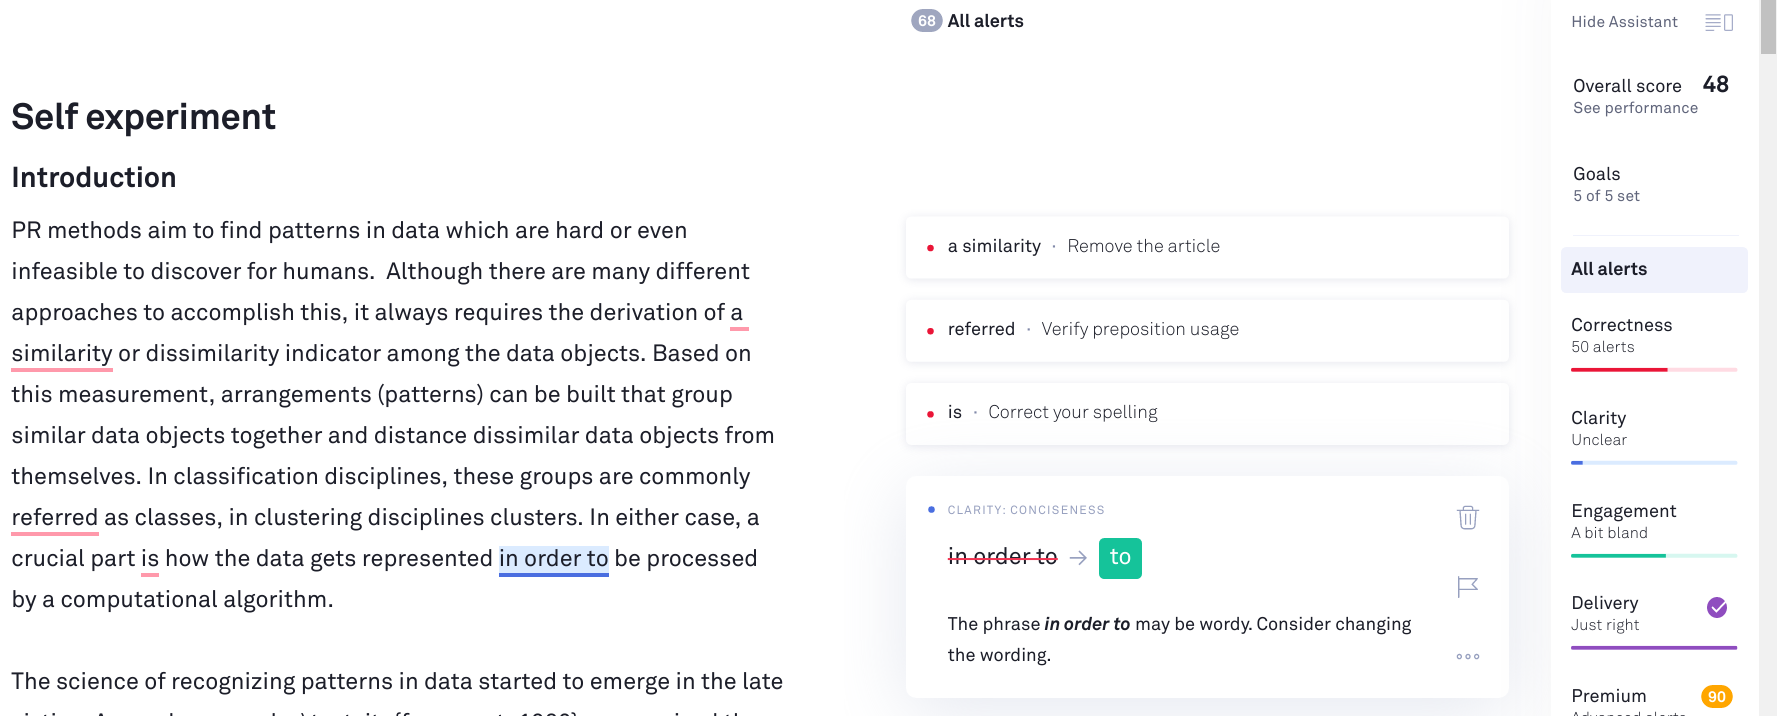
\includegraphics[width=\linewidth]{images/view.png}
  \caption{Revision view.}
  \label{fig:revision}
\end{figure}

Each feedback card can be in three different states. In the overview all the cards are in the collapsed state to not use up much space. Only the text containing an issue and a quick recommendation is displayed.

\begin{figure}[H]
  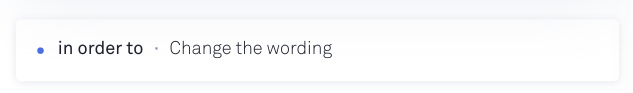
\includegraphics[width=\linewidth]{images/state_1.png}
  \caption{Collapsed state.}
  \label{fig:state1}
\end{figure}

When clicking into the underlined text section or by clicking the feedback card directly, the card expands and gives a full sentence explanation of the issue. With a simple click on the greenn correction the proposed solution can be accepted or declined by clicking the bin button.
\begin{figure}[H]
  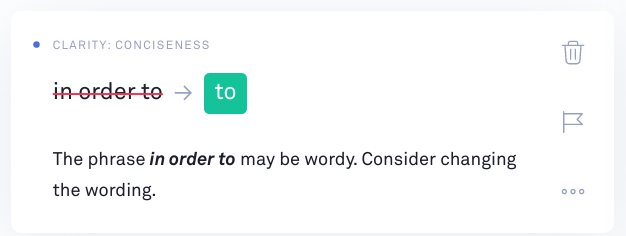
\includegraphics[width=\linewidth]{images/state_2.png}
  \caption{Extended state.}
  \label{fig:state2}
\end{figure}

If more information is still needed to make the final decision, a detailed explanation of the rule, including examples, can be displayed by clicking the three dots. 
\begin{figure}[H]
  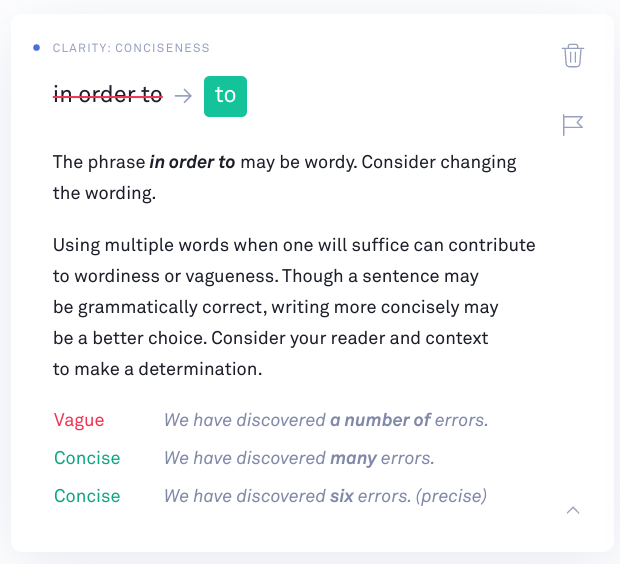
\includegraphics[width=\linewidth]{images/state_3.png}
  \caption{Detailed rule.}
  \label{fig:state3}
\end{figure}

This three stages of information help to keep the overall view organised and still show maximum information when needed. They synchronous display of the cards with the floating text make it easy to associate them together. 

\subsubsection{Revising suggestions}
While going through the various feedback cards almost all of the 68 issues could be resolved as proposed by Grammarly\textregistered. The decision if the suggested change should be applied could be done fairly quick, since the context of the sentence was always visible and could be reread quickly. The issues were so obvious that the extended feedback card was always sufficient and no further grammatical explanation was required to detect the problem. There was only one card that reported an error where there was none. 

The following issue is a false negative. The rule shown does not apply to the situation. The word ``similarity'' belongs to the term ``similarity indicator'' which is not an uncountable noun.

\say{( . . . ) it always requires the derivation of a similarity or dissimilarity indicator ( . . . )}

\noindent\fbox{%
    \parbox{\textwidth}{%
        \textbf{Feedback:} The indefinite article, \textbf{a}, may be redundant when used with the uncountable noun \textbf{similarity} in your sentence. Consider removing it.
    }%
}

After all issues have been handled, by either accepting or ignoring the suggestion the view now shows how many additional writing issues are present but can only be reviewed with a premium account.

\begin{figure}[H]
  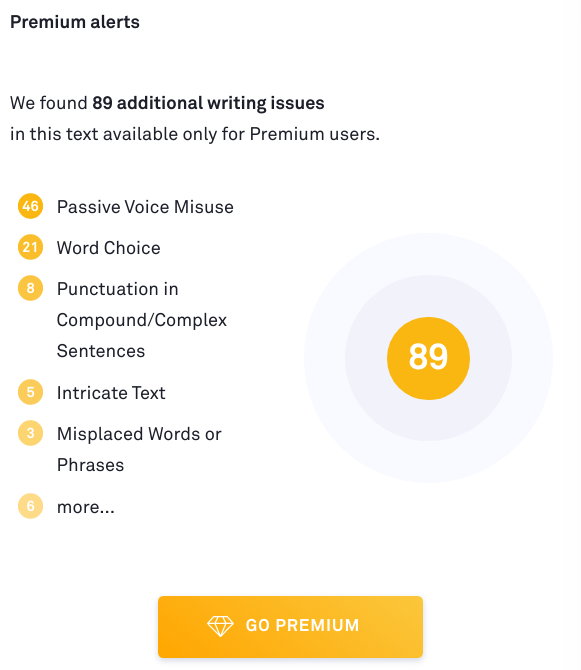
\includegraphics[width=0.8\linewidth]{images/premium.png}
  \caption{Further issues.}
  \label{fig:premium}
\end{figure}

\subsection{Discussion}
\subsubsection{Experience}
The whole revision process was smooth and the user interface was intuitive and could be managed without further documentation or explanation. Since most of the corrections could be applied as recommended this was done with the simplicity of a click. No further typing with the keyboard had to be done. The synchronous scrolling of the actual text with the cards helped immensly to keep the overview.

The progress bars in the sidebar always showed the current state of the text. While more issues were resolved those bars started to present better results which motivated even more to fix as many issues as possible. Visual components are cleverly utlised to boost the users motivation.

The user gets constantly reminded of plenty issues still present but not marked because the lack of a premium account. While also this is a very smartly placed advertisement for the payed service, it can daunt the author when he cannot make use of the full scope of improvements available.

\subsubsection{Feedback understandable}
All the issues presented in the free version of Grammarly\textregistered were easily understandable. I most cases the extended feedback card was sufficient to fully recognise the problem at hand. If I had doubt about the appropriateness of the suggestion the detailed rule helped to clarify. Specially the correct and incorrect examples made it clear how to apply a specific rule. The terminology used was understandable and did not lead to any confusion.

\subsubsection{Building new knowledge}
Specially with repeating issues that needed to be solved in the same manner over and over again, a learning effect could be detected. The iterative revisioning of the same error made this rule stick to the mind. In the further writing process the author remebers this and can think of alternative ways to construct the phrase. 

However, most of the errors seemed to be spelling or typing errors and inadvertent mistakes. Surely, Grammarly\textregistered helps to detect them and suggests corrections but it does not help avoiding them in the future. The author is usually aware of those 

The most potential for building new knowledge would have been in the areas of sentence structure, development and argumentation. However, those enahncements are not available in the free version and therefore the learning effect of the author is very limited.

\section{Discussion and recommendation}
\subsection{Overview of studies}
The automated evaluation of english texts 
pro
- quick and instant feedback
- unbiased and treating students more fairly
- provide reason for correction and facilitate learning

contra
- small range of issues 
- bad at evaluating coherence and content development, organisation
- cannot address issues / questions of the student

Does not provide the same value as face-to-face coaching 
%(dembsey_closing_2017)


\subsection{Potential benefits to FHNW students}

\subsection{Recommendation to FHNW}
- First in depth evaluation of Criterion and myaccess 
- decide to get those
- develop themselves

\section{Bibliography}


\printbibliography
\end{document}
